\section{System}
\label{sec:sys}

\begin{figure}[t]
\centering
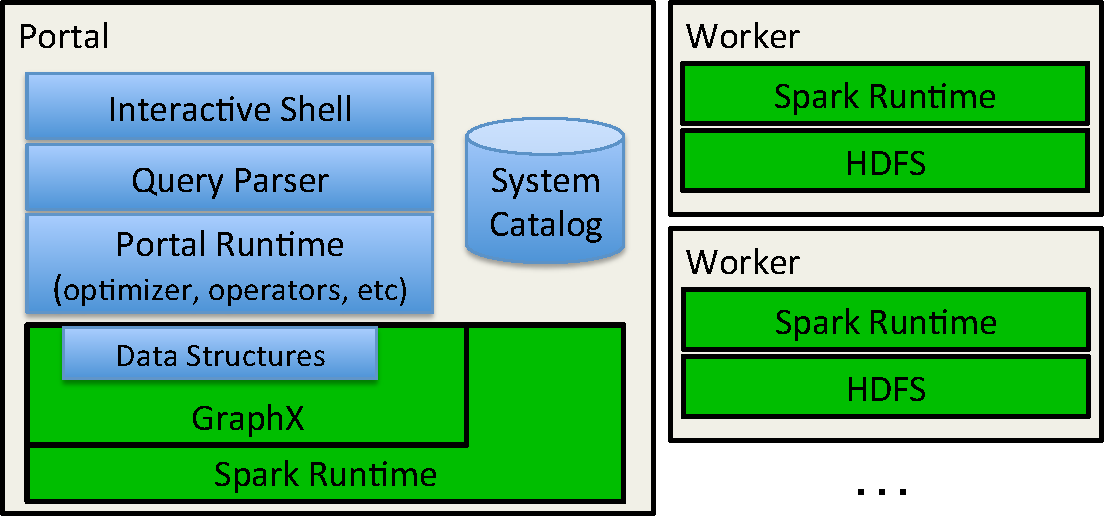
\includegraphics[width=3.4in]{figs/architecture.pdf}
\vspace{-0.4cm}
\caption{Portal system architecture.}
\vspace{-0.4cm}
\label{fig:arch}
\end{figure}

We developed a prototype system \ql which supports \tga operations on
top of Apache Spark/GraphX~\cite{DBLP:conf/osdi/GonzalezXDCFS14}, as
depicted in Figure~\ref{fig:arch}.  Green boxes indicate builtin
components, while blue are those we added for \ql.  The data is
distributed in partitions across the cluster workers, read in from
HDFS, and can be viewed both as a graph and as a pair of RDDs.  All
\tg operations are available through the public API of the \ql
library, and may be used in an Apache Spark application.

{\bf Data model.}  In~\cite{PortalarXiv2016} we proposed an evolving
graph model \tg based on temporal relations with point semantics.
Briefly, an evolving graph consists of two relations, V and E, which
represent the vertices and edges of the graph with their corresponding
intervals of validity.  Optionally, two other relations VA and EA
represent the vertex and edge attributes using the property model,
also with their periods of validity.  An example is shown in
Figure~\ref{fig:tg_rel}.

{\bf Operations.}  We also proposed a temporal graph algebra \tga
which is vertex- and edge-complete in relation to the temporal
relational algebra.  The \tga operations, some of which were shown in
the previous section, include slice, map, selection, aggregation, node
creation, edge creation, and common set operators union, intersection,
and difference.  We also support Pregel-style analytics that are
logically executed on each snapshot.

{\bf Query evaluation.}  \ql query execution follows the traditional
query processing steps: parsing, logical plan generation and
verification, and physical plan generation. \ql re-uses and extends
SparkSQL abstractions for these steps.  A \ql query is rewritten into
a sequence of operators\eat{, and some operators are reordered to
  improve performance.  For example, pushing temporal aggregation
  before temporal join can sometimes lead to better performance. A
  temporal join query may be rewritten to include additional temporal
  selection conditions, based on information about the temporal schema
  of the TGraphs being joined, which in turn significantly reduces
  data load time}.

We developed several different physical representations and
partitioning strategies that are selected at the physical plan
generation stage. The TGraphs are read from the distributed file
system HDFS and processed by Spark Workers, with the tasks assigned
and managed by the runtime.

\begin{figure}[t]
\centering
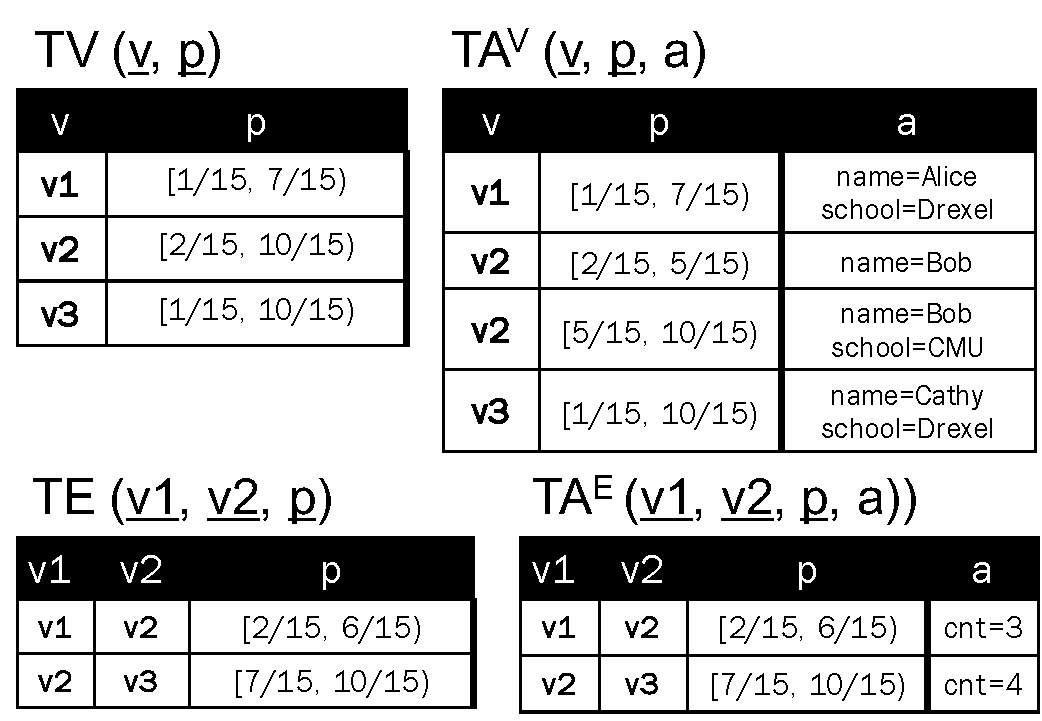
\includegraphics[width=3in]{figs/T1_rel.pdf}
\vspace{-0.2cm}
\caption{\tg \insql{T1}.}
\vspace{-0.4cm}
\label{fig:tg_rel}
\end{figure}

{\bf Interactive shell. Integration with SQL.}  The \ql system
includes an interactive shell for exploratory data analysis. Shell
users can define (materialized) views, inspect query execution plans
and execute SQL queries with an embedded \ql view. Consider the
following SQL query that returns \insql{vid} and \insql{tr} values of
20 vertices with the most significantly increasing pagerank trend.

\begin{small}
\begin{verbatim}
Select VF.vid, VF.tr
From T5.vertices() as VF
Order by tr
Limit 20
\end{verbatim}
\end{small}

An important part of the query is the use of \insql{T5.vertices()} in
the From clause. This is an operation provided by the Portal
framework, which takes all the vertices of T5 and their attributes in
a single nested relation VF with schema \insql{(vid:long, start:date,
  end:date, tr:float)}. VF can be used in SQL queries. Portal also
provides an operation \insql{edges()} that returns the edges of the
graph.



